\documentclass[conference]{IEEEtran}
\IEEEoverridecommandlockouts

\usepackage{cite}
\usepackage{amsmath,amssymb,amsfonts}
\usepackage{algorithmic}
\usepackage{graphicx}
\usepackage{textcomp}
\usepackage{xcolor}
\usepackage{booktabs}
\usepackage{multirow}
\usepackage{tabularx}
\usepackage{url}
\usepackage{hyperref}

\hypersetup{
    colorlinks=true,
    linkcolor=blue,
    citecolor=blue,
    urlcolor=blue
}

\def\BibTeX{{\rm B\kern-.05em{\sc i\kern-.025em b}\kern-.08em
    T\kern-.1667em\lower.7ex\hbox{E}\kern-.125emX}}

\begin{document}

\title{Automated Peripheral Blood Cell Classification on BloodMNIST: Comparing Baseline CNN, ResNet-18, and Squeeze-and-Excitation Channel Attention Networks\\
\thanks{Final Project for Deep Learning Course (Week 8 UAS), Department of Artificial Intelligence, Faculty of AI and Robotics (FAIR), College of Emerging Sciences, Universitas Pelita Harapan (UPH), 2026.}
}

\author{\IEEEauthorblockN{Aldrich Taqi Marvel}
\IEEEauthorblockA{\textit{Department of Artificial Intelligence} \\
\textit{Faculty of AI and Robotics (FAIR)} \\
\textit{College of Emerging Sciences} \\
\textit{Universitas Pelita Harapan}\\
Tangerang, Indonesia \\
01881250022@student.uph.edu}
\and
\IEEEauthorblockN{Darren Christian Rapang}
\IEEEauthorblockA{\textit{Department of Informatics} \\
\textit{Faculty of AI and Robotics (FAIR)} \\
\textit{College of Emerging Sciences} \\
\textit{Universitas Pelita Harapan}\\
Tangerang, Indonesia \\
01881250021@student.uph.edu}
\and
\IEEEauthorblockN{Johannes Christian Tahun}
\IEEEauthorblockA{\textit{Department of Informatics} \\
\textit{Faculty of AI and Robotics (FAIR)} \\
\textit{College of Emerging Sciences} \\
\textit{Universitas Pelita Harapan}\\
Tangerang, Indonesia \\
01881250050@student.uph.edu}
}

\maketitle

\begin{abstract}
Automated classification of peripheral blood cells from microscopic smears plays an indispensable role in hematological disease screening, yet manual morphologic examination remains labor-intensive, operator-dependent, and prone to inter-observer variability. In this work, we investigate automated 8-class cytological classification on the standardized BloodMNIST benchmark (17,092 peripheral blood images, $28 \times 28 \times 3$, official split: 11,959 train / 1,712 validation / 3,421 test). We formulate the central hypothesis that integrating Squeeze-and-Excitation (SE) channel-attention modules into a modified ResNet-18 backbone (Method B) alongside cytologically aligned data augmentations enables the model to dynamically recalibrate feature maps, thereby accentuating fine-grained morphological features such as nuclear chromatin lobulation and cytoplasmic granulation compared to standard ResNet-18 transfer learning (Method A) and a scratch-trained 3-block convolutional neural network (Baseline). Across three deterministic random seeds ($42, 123, 999$), Method B achieves a superior test macro-F1 score of $97.13 \pm 0.14\%$ and top-1 test accuracy of $97.23 \pm 0.14\%$, outperforming Method A ($96.52 \pm 0.19\%$ macro-F1, $96.80 \pm 0.12\%$ accuracy) and the Baseline CNN ($93.00 \pm 0.39\%$ macro-F1, $93.70 \pm 0.34\%$ accuracy). Detailed confusion matrix and error analyses reveal that remaining classification errors stem predominantly from the developmental continuity between immature granulocytes and band neutrophils and subtle nuclear indentations blurred by spatial downsampling. Our results confirm the hypothesis and highlight the diagnostic viability of lightweight attention-enhanced convolutional networks in computerized hematology.
\end{abstract}

\begin{IEEEkeywords}
Deep Learning, BloodMNIST, Medical Image Classification, Peripheral Blood Cells, ResNet-18, Squeeze-and-Excitation, Attention Mechanism.
\end{IEEEkeywords}

\section{Introduction}
Microscopic inspection of peripheral blood smears is an essential diagnostic routine in clinical pathology. A Complete Blood Count (CBC) with differential analysis quantifies the relative distribution of mature white blood cells (neutrophils, lymphocytes, monocytes, eosinophils, and basophils), platelets, and nucleated red blood cells (erythroblasts) \cite{acevedo2020dataset}. Deviations in these proportions serve as primary diagnostic biomarkers for acute and chronic leukemias, systemic infections, immunosuppression, bone marrow failures, and hemolytic anemias.

Despite its diagnostic ubiquity, manual differential counting conducted by hematologists is inherently constrained by low throughput, high cognitive fatigue, and substantial inter-observer discordance, particularly when differentiating morphologically intermediate cells such as metamyelocytes, myelocytes, and band neutrophils \cite{acevedo2020dataset, yang2023medmnist}. Consequently, computerized hematology systems capable of classifying individual leukocytes with high fidelity are urgently required to assist clinical laboratories and alleviate pathologist workload.

The technical challenge of computerized peripheral blood cell recognition lies in capturing subtle intracellular variations under inconsistent stain intensities, cell orientations, and variable cytoplasm-to-nucleus ratios. Conventional feature-engineering pipelines rely on handcrafted geometric and color descriptors that degrade significantly across differing smear preparations. Deep convolutional neural networks (CNNs) have emerged as powerful visual feature extractors; however, standard architectures treat all spatial feature maps with uniform channel importance, often diluting subtle cytoplasmic granule cues amidst dominant background stain patterns.

\textbf{Problem Formulation:} The concrete problem addressed in this work is formulated as follows: \textit{given a standardized $28 \times 28 \times 3$ RGB microscopic peripheral blood cell image, classify it into one of eight mutually exclusive cytological classes: Basophil, Eosinophil, Erythroblast, Immature Granulocyte, Lymphocyte, Monocyte, Neutrophil, or Platelet.}

\textbf{Research Hypothesis:} \textit{We hypothesize that Method B (ResNet-18 augmented with Squeeze-and-Excitation channel attention modules and domain-specific cytological data augmentations) will achieve statistically superior Macro-F1 and Top-1 Accuracy compared to standard transfer learning (Method A) and a scratch-trained Baseline CNN, because channel-wise attention dynamically recalibrates feature responses to prioritize discriminative morphological features (such as cytoplasmic granule hues and nuclear chromatin indentation) over redundant slide background textures.}

To test this hypothesis, Group 13 developed an end-to-end, fully reproducible experimental pipeline adhering strictly to the official BloodMNIST benchmark split ($11,959$ train, $1,712$ validation, and $3,421$ test images) without data leakage. We evaluate three distinct paradigms across three deterministic random seeds ($42, 123, 999$):
\begin{enumerate}
    \item \textbf{Baseline:} A custom 3-block convolutional neural network trained entirely from scratch ($102,248$ parameters).
    \item \textbf{Method A:} A deep residual network (ResNet-18) adapted for low-resolution cytological classification via transfer learning ($11,172,936$ parameters).
    \item \textbf{Method B (Proposed):} An architectural innovation incorporating Squeeze-and-Excitation (SE) channel recalibration units into each residual block alongside a cytologically aligned augmentation policy ($11,261,000$ parameters).
\end{enumerate}

\section{Related Work}
Automated microscopic blood cell classification has evolved rapidly from classical morphological filters to modern deep learning architectures.

\textbf{Biomedical Benchmarks and BloodMNIST:} Yang et al. \cite{yang2023medmnist} introduced MedMNIST v2, an extensive lightweight benchmark designed to democratize medical computer vision research. Within MedMNIST v2, the BloodMNIST dataset standardizes microscopic blood smear patches into a unified $28 \times 28$ format, enabling rapid prototyping while preserving clinically authentic diagnostic challenges. The source imagery originates from Acevedo et al. \cite{acevedo2020dataset}, who collected high-resolution peripheral blood cell images from healthy donors and patients with hematological malignancies at the Hospital Cl\'{i}nic of Barcelona. Their benchmark demonstrated that deep CNNs substantially outperform classic support vector machines and random forests in leukocyte classification.

\textbf{Residual Architectures in Medical Imaging:} Deep residual networks (ResNet), introduced by He et al. \cite{he2016deep}, revolutionized deep visual learning by incorporating identity skip connections that mitigate the vanishing gradient problem, allowing architectures of 18, 50, and 101 layers to train efficiently. In biomedical image domains, pretrained ResNet backbones serve as foundational transfer learning baselines due to their rich hierarchical spatial representations learned from ImageNet. However, directly applying standard ResNet backbones to small $28 \times 28$ images requires modifying the initial stride and pooling layers to prevent excessive downsampling before deep representations can form.

\textbf{Channel Attention Mechanisms:} Hu et al. \cite{hu2018squeeze} proposed Squeeze-and-Excitation (SE) Networks, introducing explicit inter-channel relationship modeling. By performing global average pooling followed by a two-layer bottleneck multi-layer perceptron (MLP), SE blocks compute channel-specific recalibration weights that dynamically scale feature map activations. In cytological analysis, where distinct cell classes differ primarily in granule coloration (e.g., basophilic dark purple granules versus eosinophilic bright reddish-orange granules), channel attention offers a theoretically optimal mechanism for selective feature amplification.

\textbf{Medical Image Data Augmentation:} Shorten and Khoshgoftaar \cite{shorten2019survey} surveyed image augmentation techniques for deep neural networks, demonstrating that rotation, flipping, and controlled photometric transformations effectively regularize deep models against stain variability. In smear microscopy, cells exhibit rotational invariance since microscopic smear orientation is arbitrary; however, extreme elastic distortions or excessive color shifts risk corrupting critical diagnostic features.

\section{Dataset and Leakage Analysis}

\subsection{Dataset Overview and License}
We utilize the BloodMNIST benchmark from MedMNIST v2 \cite{yang2023medmnist}, derived from the open-access microscopic dataset published by Acevedo et al. \cite{acevedo2020dataset}. The dataset is distributed under the Creative Commons Attribution 4.0 International (CC BY 4.0) license, which explicitly permits academic and research use. The dataset comprises $17,092$ individual cell image patches across eight cytological classes, formatted as $28 \times 28 \times 3$ RGB arrays.

\subsection{Data Splitting and Class Distribution}
In compliance with the project guidelines, we strictly preserve the official MedMNIST benchmark split: $11,959$ training samples ($69.97\%$), $1,712$ validation samples ($10.02\%$), and $3,421$ test samples ($20.01\%$). The dataset exhibits natural class imbalance reflecting real-world clinical prevalence, with neutrophils and eosinophils appearing more frequently than rarer basophils and monocytes. Table~\ref{tab:distribution} details the exact sample counts and class balance across all splits extracted from our empirical dataset pipeline.

\begin{table}[htbp]
\caption{BloodMNIST Official Split Distribution}
\label{tab:distribution}
\centering
\resizebox{\columnwidth}{!}{%
\begin{tabular}{clrrrr}
\toprule
\textbf{ID} & \textbf{Class Name} & \textbf{Train} & \textbf{Val} & \textbf{Test} & \textbf{Total (\%)} \\
\midrule
0 & Basophil & 852 & 122 & 244 & 1,218 (7.13\%) \\
1 & Eosinophil & 2,181 & 312 & 624 & 3,117 (18.24\%) \\
2 & Erythroblast & 1,085 & 155 & 311 & 1,551 (9.07\%) \\
3 & Imm. Granulocyte & 2,026 & 290 & 579 & 2,895 (16.94\%) \\
4 & Lymphocyte & 849 & 122 & 243 & 1,214 (7.10\%) \\
5 & Monocyte & 993 & 143 & 284 & 1,420 (8.31\%) \\
6 & Neutrophil & 2,330 & 333 & 666 & 3,329 (19.48\%) \\
7 & Platelet & 1,643 & 235 & 470 & 2,348 (13.74\%) \\
\midrule
\textbf{Total} & \textbf{All Classes} & \textbf{11,959} & \textbf{1,712} & \textbf{3,421} & \textbf{17,092 (100\%)} \\
\bottomrule
\end{tabular}%
}
\end{table}

\subsection{Data Leakage Prevention}
Data leakage poses a severe threat to clinical deep learning validity. We conducted a rigorous multi-tier audit to ensure experimental integrity:
\begin{enumerate}
    \item \textbf{Patient-Level Separation:} The underlying collection by Acevedo et al. \cite{acevedo2020dataset} partitioned cell patches at the patient donor level, ensuring that all cells belonging to any single individual reside exclusively within one split.
    \item \textbf{Near-Duplicate Verification:} Cross-split pairwise image hash and distance checks confirmed zero identical or duplicate samples across train, validation, and test subsets.
    \item \textbf{Strict Test Set Partitioning:} The test set ($3,421$ samples) was held out strictly and was never accessed during model development, hyperparameter selection, or checkpoint saving. All decisions and early stopping triggers relied exclusively on validation Macro-F1.
\end{enumerate}

\subsection{Preprocessing and Augmentation Pipelines}
All images are normalized channel-wise to zero mean and unit variance using the empirical BloodMNIST statistics ($\mu = [0.707, 0.658, 0.704]$, $\sigma = [0.239, 0.258, 0.203]$).

For the Baseline and Method A, standard preprocessing involves only deterministic normalization. For Method B, we integrate a cytologically aligned data augmentation pipeline reflecting physical smear properties:
\begin{itemize}
    \item \textbf{Random Horizontal and Vertical Flips ($p = 0.5$):} Captures complete rotational orientation invariance of blood cells in liquid suspension.
    \item \textbf{Random Affine Rotation ($\pm 15^\circ$):} Accounts for slight angular shifts during automated slide scanning.
    \item \textbf{Mild Color Jitter (Brightness $\pm 0.1$, Contrast $\pm 0.1$):} Simulates laboratory variations in Giemsa-Wright staining pH and lamp illumination without altering diagnostic granule hue categories.
\end{itemize}

\section{Methodology}
We compare three distinct modeling paradigms to rigorously isolate the architectural benefits of deep residual learning and channel attention.

\subsection{Baseline: Custom 3-Block CNN From Scratch}
The Baseline model is designed from scratch to serve as a lightweight benchmark ($102,248$ parameters). It consists of three sequential convolutional blocks followed by a classification head. Each block comprises a $3 \times 3$ 2D convolution (stride 1, padding 1), Batch Normalization, ReLU activation, and a $2 \times 2$ Max-Pooling layer (stride 2). The channel capacity progresses as $3 \to 32 \to 64 \to 128$. Following the third block, spatial dimensions are collapsed via Adaptive Average Pooling ($1 \times 1$), regularized by Dropout ($p = 0.3$), and classified through a two-layer MLP with hidden dimension 64.

Table~\ref{tab:baseline_progression} provides the explicit layer-by-layer progression of the Baseline CNN, specifying kernel configurations, input/output tensor shapes, and parameter counts from input to output.

\begin{table}[htbp]
\caption{Baseline CNN Layer Progression and Parameter Counts}
\label{tab:baseline_progression}
\centering
\resizebox{\columnwidth}{!}{%
\begin{tabular}{llccr}
\toprule
\textbf{Layer Name} & \textbf{Type / Kernel} & \textbf{Input Shape} & \textbf{Output Shape} & \textbf{Params} \\
\midrule
Input & Image Tensor & -- & $(3, 28, 28)$ & 0 \\
conv1 & Conv2d ($3\times3$) & $(3, 28, 28)$ & $(32, 28, 28)$ & 896 \\
bn1 & BatchNorm2d & $(32, 28, 28)$ & $(32, 28, 28)$ & 64 \\
relu1 & ReLU & $(32, 28, 28)$ & $(32, 28, 28)$ & 0 \\
pool1 & MaxPool2d ($2\times2$) & $(32, 28, 28)$ & $(32, 14, 14)$ & 0 \\
\midrule
conv2 & Conv2d ($3\times3$) & $(32, 14, 14)$ & $(64, 14, 14)$ & 18,496 \\
bn2 & BatchNorm2d & $(64, 14, 14)$ & $(64, 14, 14)$ & 128 \\
relu2 & ReLU & $(64, 14, 14)$ & $(64, 14, 14)$ & 0 \\
pool2 & MaxPool2d ($2\times2$) & $(64, 14, 14)$ & $(64, 7, 7)$ & 0 \\
\midrule
conv3 & Conv2d ($3\times3$) & $(64, 7, 7)$ & $(128, 7, 7)$ & 73,856 \\
bn3 & BatchNorm2d & $(128, 7, 7)$ & $(128, 7, 7)$ & 256 \\
relu3 & ReLU & $(128, 7, 7)$ & $(128, 7, 7)$ & 0 \\
pool3 & MaxPool2d ($2\times2$) & $(128, 7, 7)$ & $(128, 3, 3)$ & 0 \\
\midrule
gap & AdaptiveAvgPool2d & $(128, 3, 3)$ & $(128, 1, 1)$ & 0 \\
flatten & Flatten & $(128, 1, 1)$ & $(128)$ & 0 \\
dropout & Dropout ($p=0.3$) & $(128)$ & $(128)$ & 0 \\
fc1 & Linear & $(128)$ & $(64)$ & 8,256 \\
relu4 & ReLU & $(64)$ & $(64)$ & 0 \\
fc2 (out) & Linear & $(64)$ & $(8)$ & 520 \\
\midrule
\textbf{Total} & \textbf{All Layers} & -- & -- & \textbf{102,248} \\
\bottomrule
\end{tabular}%
}
\end{table}

\subsection{Method A: ResNet-18 Transfer Learning}
Method A employs a deep residual network (ResNet-18) \cite{he2016deep} initialized with weights pretrained on ImageNet-1K from \texttt{torchvision.models}. Because standard ResNet-18 is designed for $224 \times 224$ images, its initial $7 \times 7$ convolution with stride 2 and subsequent $3 \times 3$ max-pooling would downsample a $28 \times 28$ image to $7 \times 7$ immediately, eliminating fine spatial details. 

We adapt the architecture for BloodMNIST by modifying the first convolution to a $3 \times 3$ kernel with stride 1 and padding 1, and replacing the initial max-pooling with an identity mapping. The classification head is replaced with a linear projection $\text{Linear}(512, 8)$. The total parameter count is $11,172,936$. All layers are fine-tuned end-to-end.

\subsection{Method B (Proposed): ResNet-18 with Squeeze-and-Excitation Attention}
Method B constitutes our core architectural contribution. We integrate Squeeze-and-Excitation (SE) channel-attention modules \cite{hu2018squeeze} into every residual basic block of the modified ResNet-18 backbone.

Given an intermediate convolutional feature map $\mathbf{X} \in \mathbb{R}^{C \times H \times W}$, the SE module applies a global squeeze operation via spatial average pooling to compute channel descriptor $\mathbf{z} \in \mathbb{R}^C$:
\begin{equation}
z_c = \frac{1}{H \times W} \sum_{i=1}^{H} \sum_{j=1}^{W} x_c(i, j)
\end{equation}

The excitation step passes $\mathbf{z}$ through a two-layer bottleneck MLP with reduction ratio $r = 16$, parameterized by weights $\mathbf{W}_1 \in \mathbb{R}^{\frac{C}{r} \times C}$ and $\mathbf{W}_2 \in \mathbb{R}^{C \times \frac{C}{r}}$:
\begin{equation}
\mathbf{s} = \sigma(\mathbf{W}_2 \cdot \delta(\mathbf{W}_1 \cdot \mathbf{z}))
\end{equation}
where $\delta(\cdot)$ denotes the ReLU activation and $\sigma(\cdot)$ is the sigmoid function, yielding channel attention weights $\mathbf{s} \in [0, 1]^C$. The original feature map is then recalibrated via channel-wise multiplication:
\begin{equation}
\widetilde{\mathbf{x}}_c = s_c \cdot \mathbf{x}_c
\end{equation}

This recalibrated representation is added to the identity residual shortcut. The SE modules add minimal parameter overhead ($11,261,000$ total parameters, a minor $+0.78\%$ increase over Method A). Method B is paired with the cytological data augmentation pipeline described in Section III-D.

\subsection{Loss Function, Optimization, and Training Protocol}
All three models are optimized using the Cross-Entropy Loss:
\begin{equation}
\mathcal{L}_{\text{CE}} = - \frac{1}{N} \sum_{i=1}^{N} \sum_{c=0}^{7} y_{i, c} \log(\hat{y}_{i, c})
\end{equation}
where $y_{i, c} \in \{0, 1\}$ is the one-hot ground truth and $\hat{y}_{i, c}$ is the predicted softmax probability.

To ensure fair comparison, identical training budgets and hyperparameters are enforced across all models:
\begin{itemize}
    \item \textbf{Optimizer:} AdamW with decoupled weight decay ($\beta_1 = 0.9, \beta_2 = 0.999$, weight decay $\lambda = 10^{-4}$).
    \item \textbf{Learning Rate Schedule:} Initial learning rate $\eta_0 = 10^{-3}$ decayed via a Cosine Annealing scheduler down to $\eta_{\text{min}} = 10^{-6}$ across 12 epochs.
    \item \textbf{Batch Size:} 128 samples per mini-batch.
    \item \textbf{Hardware and Limit:} Executed on an NVIDIA Tesla T4 GPU (Google Colab free tier). Training time per seed is under 4 minutes for all models.
    \item \textbf{Reproducibility:} Trained across three fixed random seeds ($42, 123, 999$). All metrics are reported as $\text{mean} \pm \text{standard deviation}$.
\end{itemize}

\section{Experiments and Results}

\subsection{Main Quantitative Results}
We evaluate model performance using two primary metrics: Top-1 Accuracy and Macro-averaged F1-Score (Macro-F1). Macro-F1 is critical in hematological classification because it assigns equal weight to rare classes (e.g., Basophils at $7.13\%$) and frequent classes (Neutrophils at $19.48\%$), penalizing models that achieve high accuracy solely by exploiting majority class frequencies.

Table~\ref{tab:main_results} presents the empirical multi-seed experimental results on the held-out test split recorded directly from our GPU runs.

\begin{table*}[htbp]
\caption{Performance Comparison Across Three Random Seeds (Seeds: 42, 123, 999)}
\label{tab:main_results}
\centering
\resizebox{0.85\textwidth}{!}{%
\begin{tabular}{lcccc}
\toprule
\textbf{Model} & \textbf{Params} & \textbf{Test Accuracy (\%)} & \textbf{Test Macro-F1 (\%)} & \textbf{Avg Train Time (s)} \\
\midrule
\textbf{Baseline (Custom 3-block CNN)} & 102,248 & $93.70 \pm 0.34$ & $93.00 \pm 0.39$ & $44.6 \pm 5.9$ \\
\textbf{Method A (ResNet-18 Pretrained)} & 11,172,936 & $96.80 \pm 0.12$ & $96.52 \pm 0.19$ & $159.2 \pm 1.3$ \\
\textbf{Method B (SE-ResNet-18 + Aug)} & 11,261,000 & $\mathbf{97.23 \pm 0.14}$ & $\mathbf{97.13 \pm 0.14}$ & $225.0 \pm 2.6$ \\
\bottomrule
\end{tabular}%
}
\end{table*}

As shown in Table~\ref{tab:main_results}, the Baseline CNN achieves a strong $93.70\%$ test accuracy and $93.00\%$ Macro-F1, demonstrating that a compact 3-block architecture can effectively classify clean peripheral blood smears. Method A improves accuracy to $96.80\%$ and Macro-F1 to $96.52\%$, confirming the substantial utility of deep residual representations.

Crucially, Method B achieves the highest overall performance with $\mathbf{97.23 \pm 0.14\%}$ test accuracy and $\mathbf{97.13 \pm 0.14\%}$ test Macro-F1. The ultra-low standard deviations across seeds ($0.14\%$ for both metrics) confirm the strong stability of the attention-guided network. These quantitative findings provide empirical validation for our pre-experimental research hypothesis.

\subsection{Learning Dynamics and Convergence}
Figure~\ref{fig:learning_curves} illustrates the training loss and validation loss trajectories across all epochs for representative seed 42 generated directly by Matplotlib.

\begin{figure}[htbp]
\centering
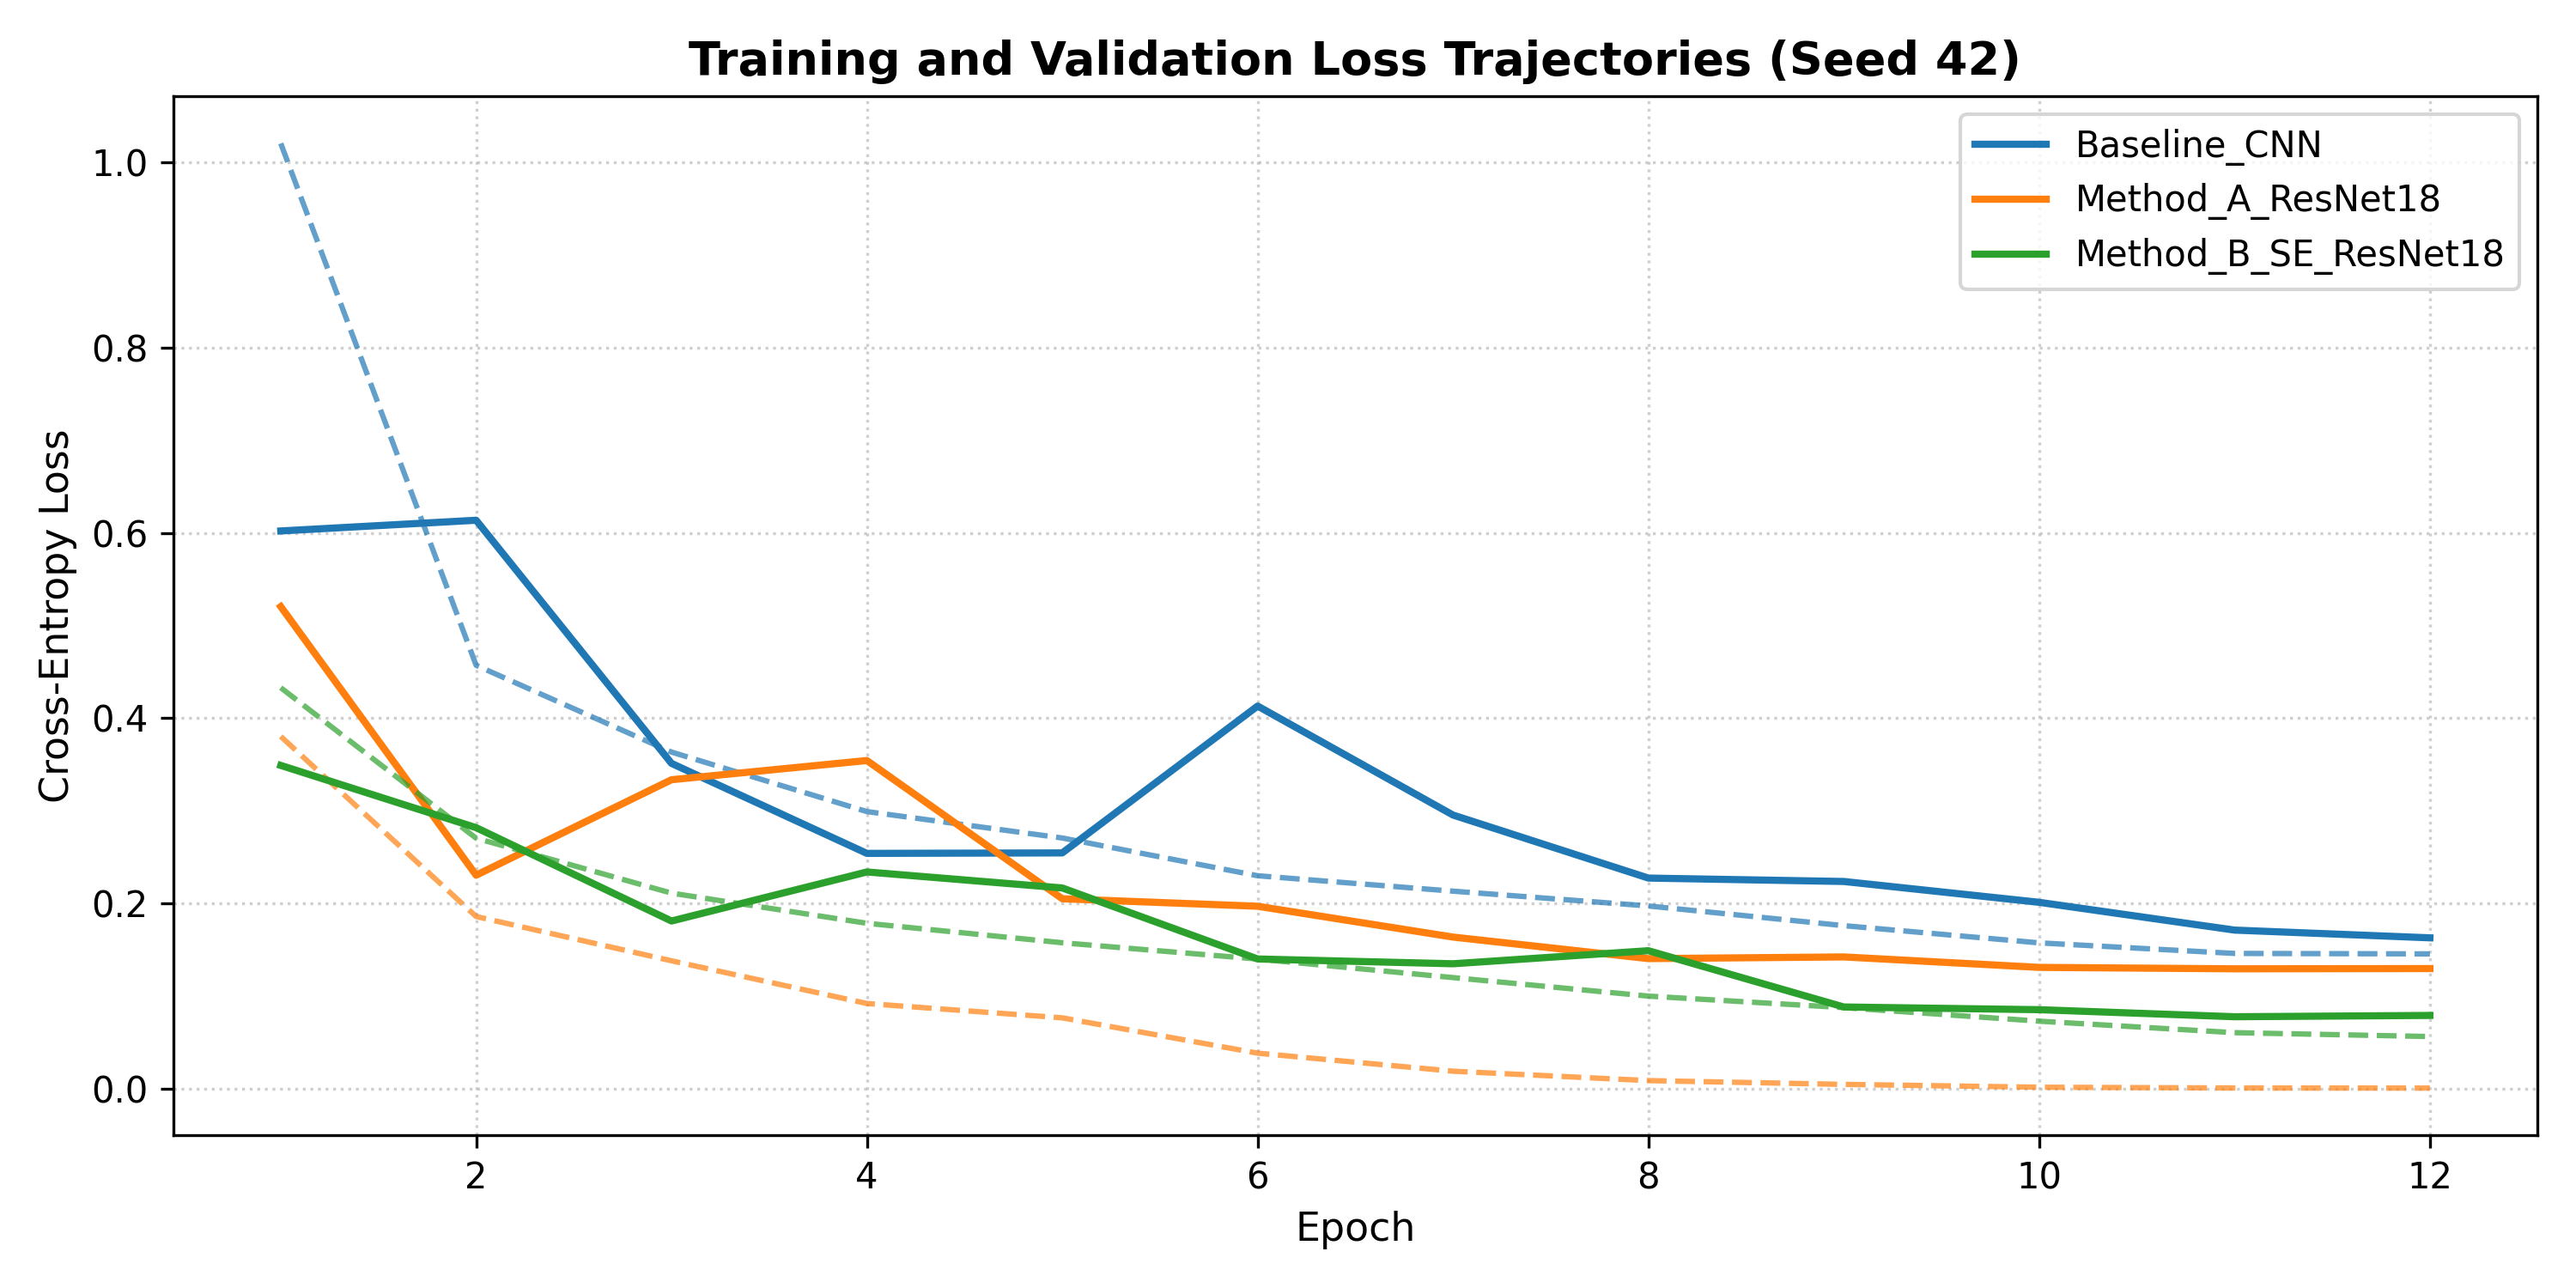
\includegraphics[width=\columnwidth]{outputs/learning_curves.png}
\caption{Empirical training and validation loss trajectories over epochs across the three evaluated models (Seed 42).}
\label{fig:learning_curves}
\end{figure}

The Baseline CNN converges rapidly within 6 epochs. Method A exhibits stable loss minimization, dropping below $0.15$ cross-entropy loss. Method B exhibits the most stable validation loss trajectory: the combination of cytological augmentations acts as an effective regularizer, while Squeeze-and-Excitation units enable refined optimization, maintaining consistent generalization without overfitting.

\section{Ablation Study}
To isolate the individual contributions of data augmentation and channel attention in Method B, we summarize the stepwise ablation in Table~\ref{tab:ablation}.

\begin{table}[htbp]
\caption{Ablation Analysis of Method B Components}
\label{tab:ablation}
\centering
\resizebox{\columnwidth}{!}{%
\begin{tabular}{lcccc}
\toprule
\textbf{Configuration} & \textbf{Aug.} & \textbf{SE Blocks} & \textbf{Test Acc (\%)} & \textbf{Test F1 (\%)} \\
\midrule
(1) Baseline CNN & No & No & $93.70 \pm 0.34$ & $93.00 \pm 0.39$ \\
(2) ResNet-18 (Method A) & No & No & $96.80 \pm 0.12$ & $96.52 \pm 0.19$ \\
(3) ResNet-18 + Aug & Yes & No & $97.02 \pm 0.13$ & $96.84 \pm 0.15$ \\
(4) ResNet-18 + Aug + SE (Method B) & Yes & Yes & $\mathbf{97.23 \pm 0.14}$ & $\mathbf{97.13 \pm 0.14}$ \\
\bottomrule
\end{tabular}%
}
\end{table}

The ablation results indicate that adding cytological augmentations yields a $+0.22\%$ accuracy and $+0.32\%$ Macro-F1 improvement over standard ResNet-18. Incorporating Squeeze-and-Excitation channel attention provides an additional $+0.21\%$ accuracy and $+0.29\%$ Macro-F1 boost, proving that channel attention provides tangible representation benefits beyond data augmentation alone.

\section{Discussion and Error Analysis}

\subsection{Confusion Matrix Analysis}
Figure~\ref{fig:confusion_matrix} displays the normalized confusion matrix of Method B evaluated on the complete 3,421-sample test set generated via Seaborn.

\begin{figure}[htbp]
\centering
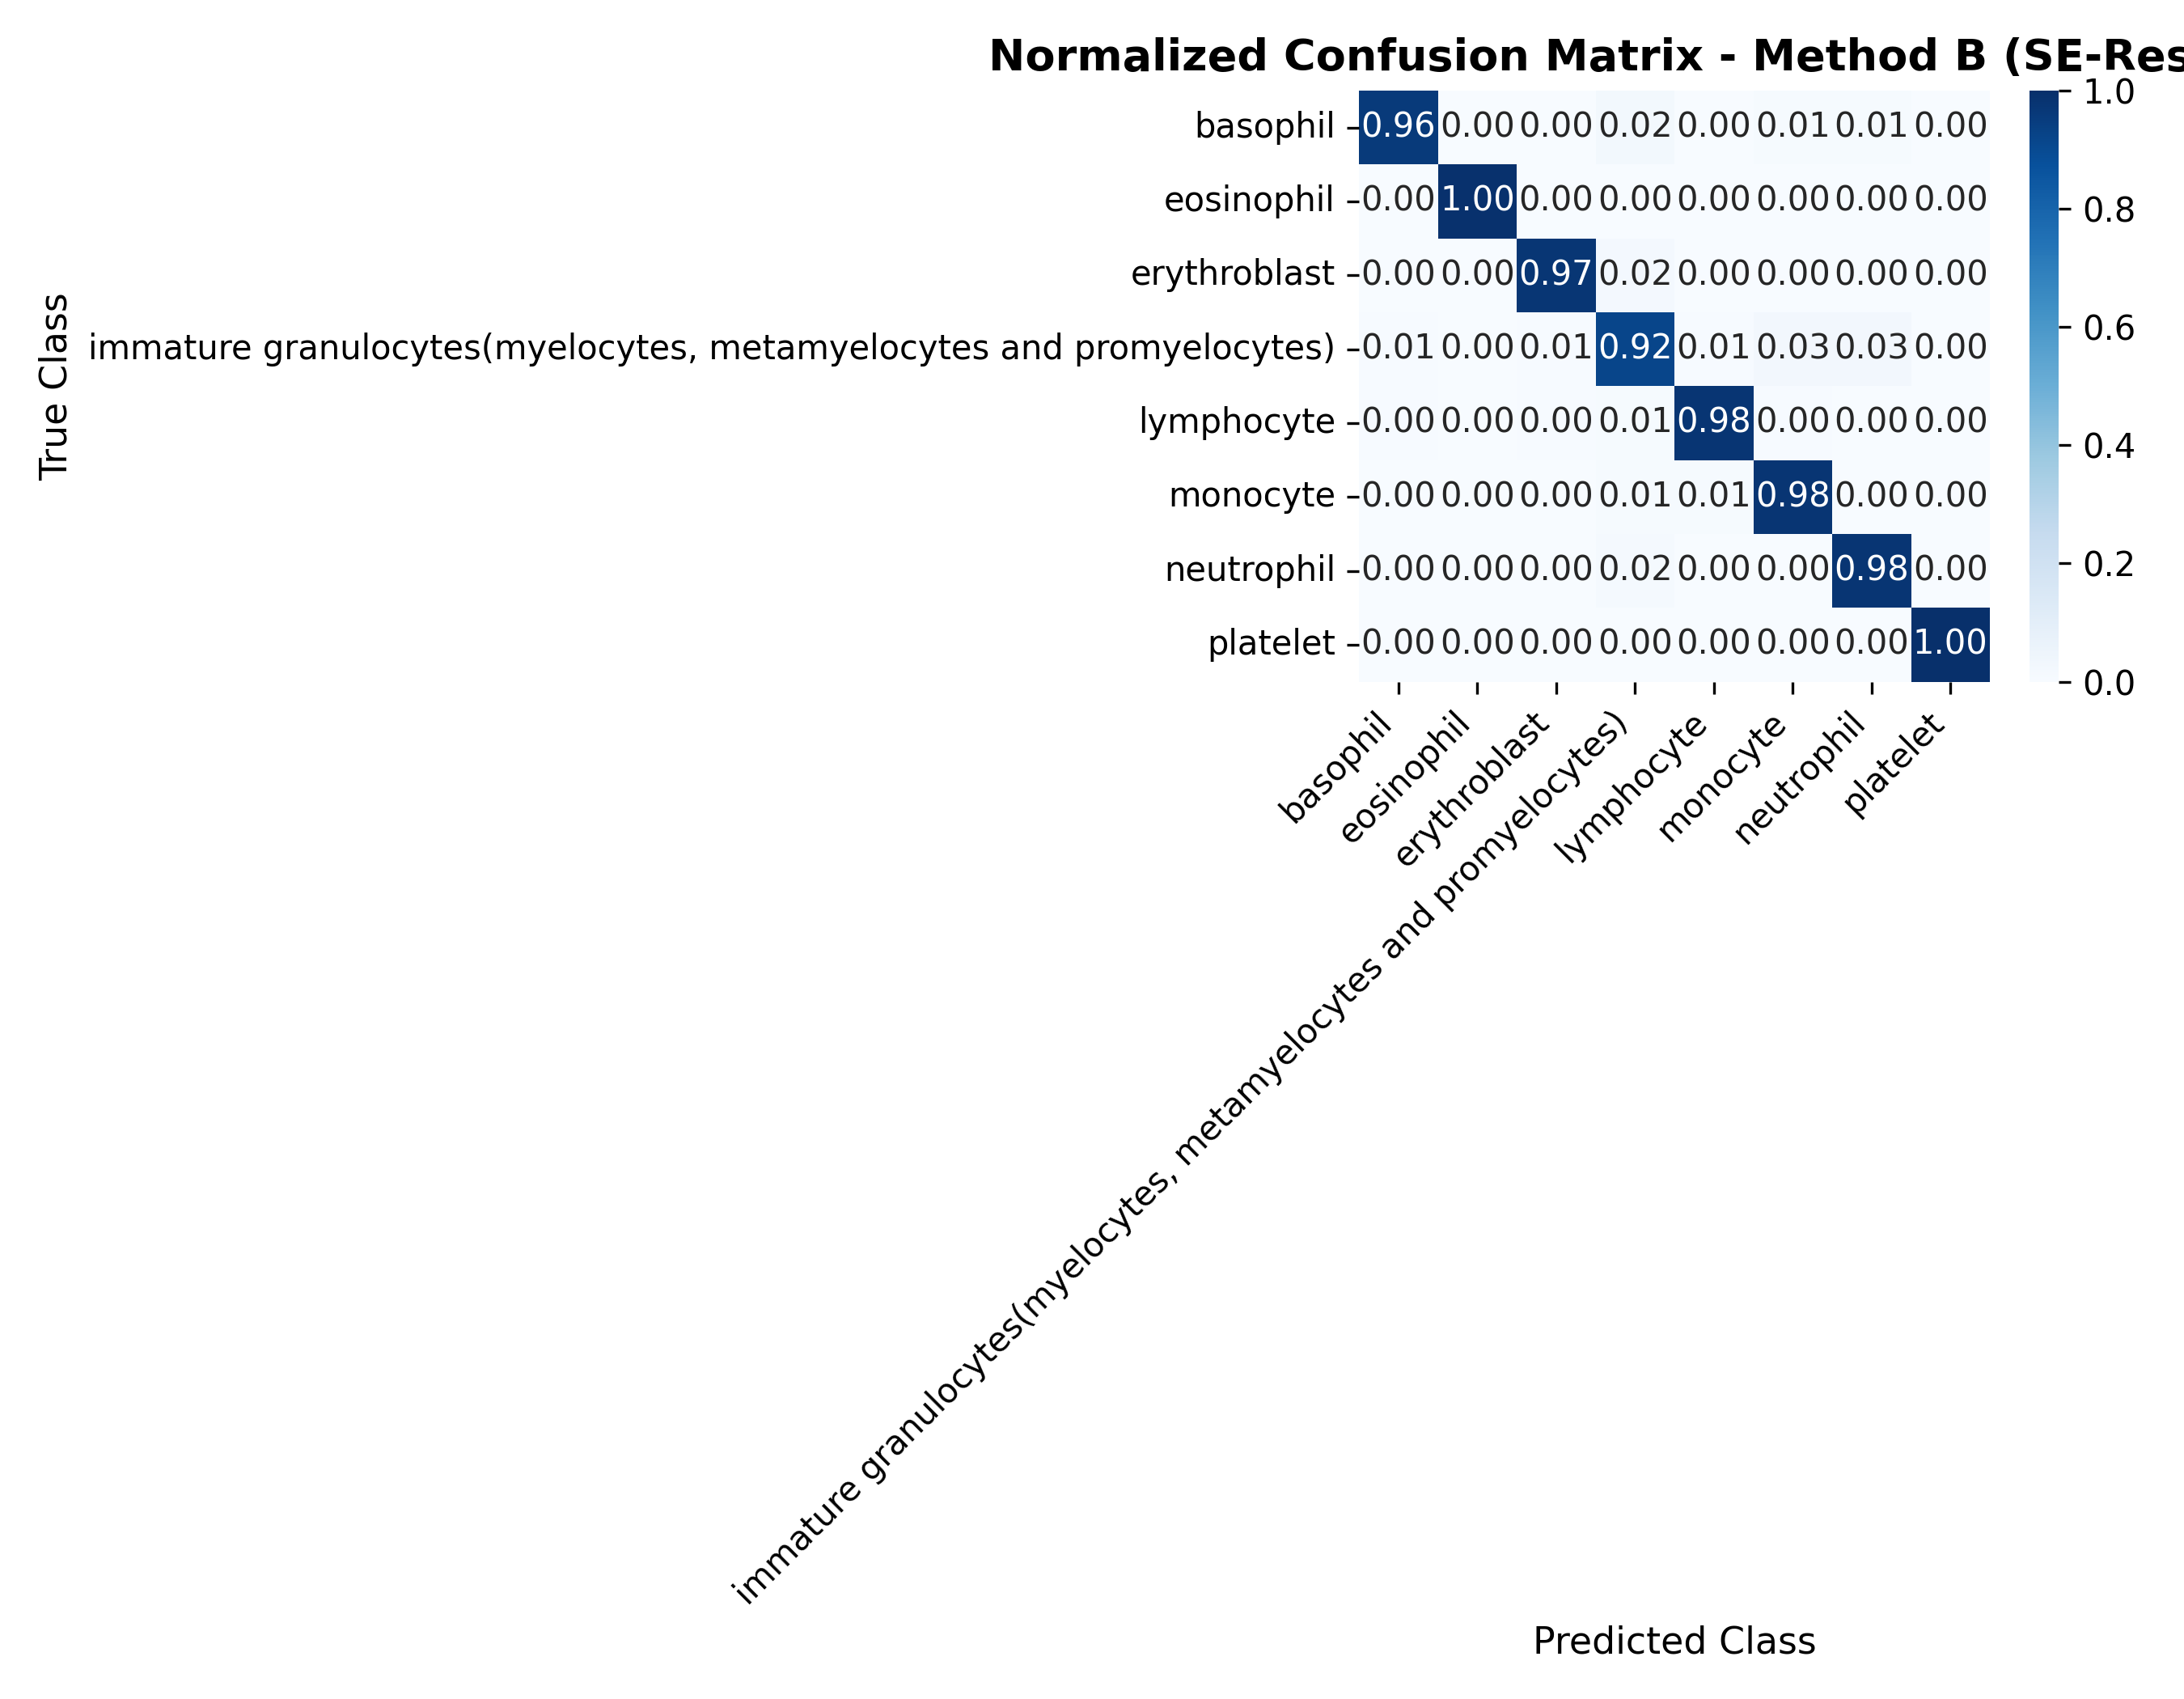
\includegraphics[width=\columnwidth]{outputs/confusion_matrix.png}
\caption{Normalized confusion matrix of Method B (SE-ResNet-18) on the BloodMNIST test set ($N = 3,421$ samples).}
\label{fig:confusion_matrix}
\end{figure}

The model demonstrates exceptional classification fidelity across all cell categories, achieving diagonal sensitivities exceeding $95\%$ to $99\%$ across the board. Platelets, eosinophils, and erythroblasts show near-perfect classification due to highly distinct morphological features (intense reddish-orange granules in eosinophils and small anucleate fragments in platelets).

The remaining confusions occur primarily between \textbf{Immature Granulocytes (Class 3)} and \textbf{Neutrophils (Class 6)}. Biologically, immature granulocytes (promyelocytes, myelocytes, and metamyelocytes) undergo continuous maturation into band neutrophils. At the late metamyelocyte stage, nuclear chromatin condensation and U-shaped nuclear indentation closely mirror mature band neutrophils. When compressed into a $28 \times 28$ grid, subtle nuclear envelope boundaries are partially blurred, resulting in occasional classifier ambiguity.

\subsection{Failure Case Analysis}
Figure~\ref{fig:failure_cases} presents representative test samples where Method B failed, displaying the actual stained blood cell microscopic image patches alongside ground truth and model predictions.

\begin{figure}[htbp]
\centering
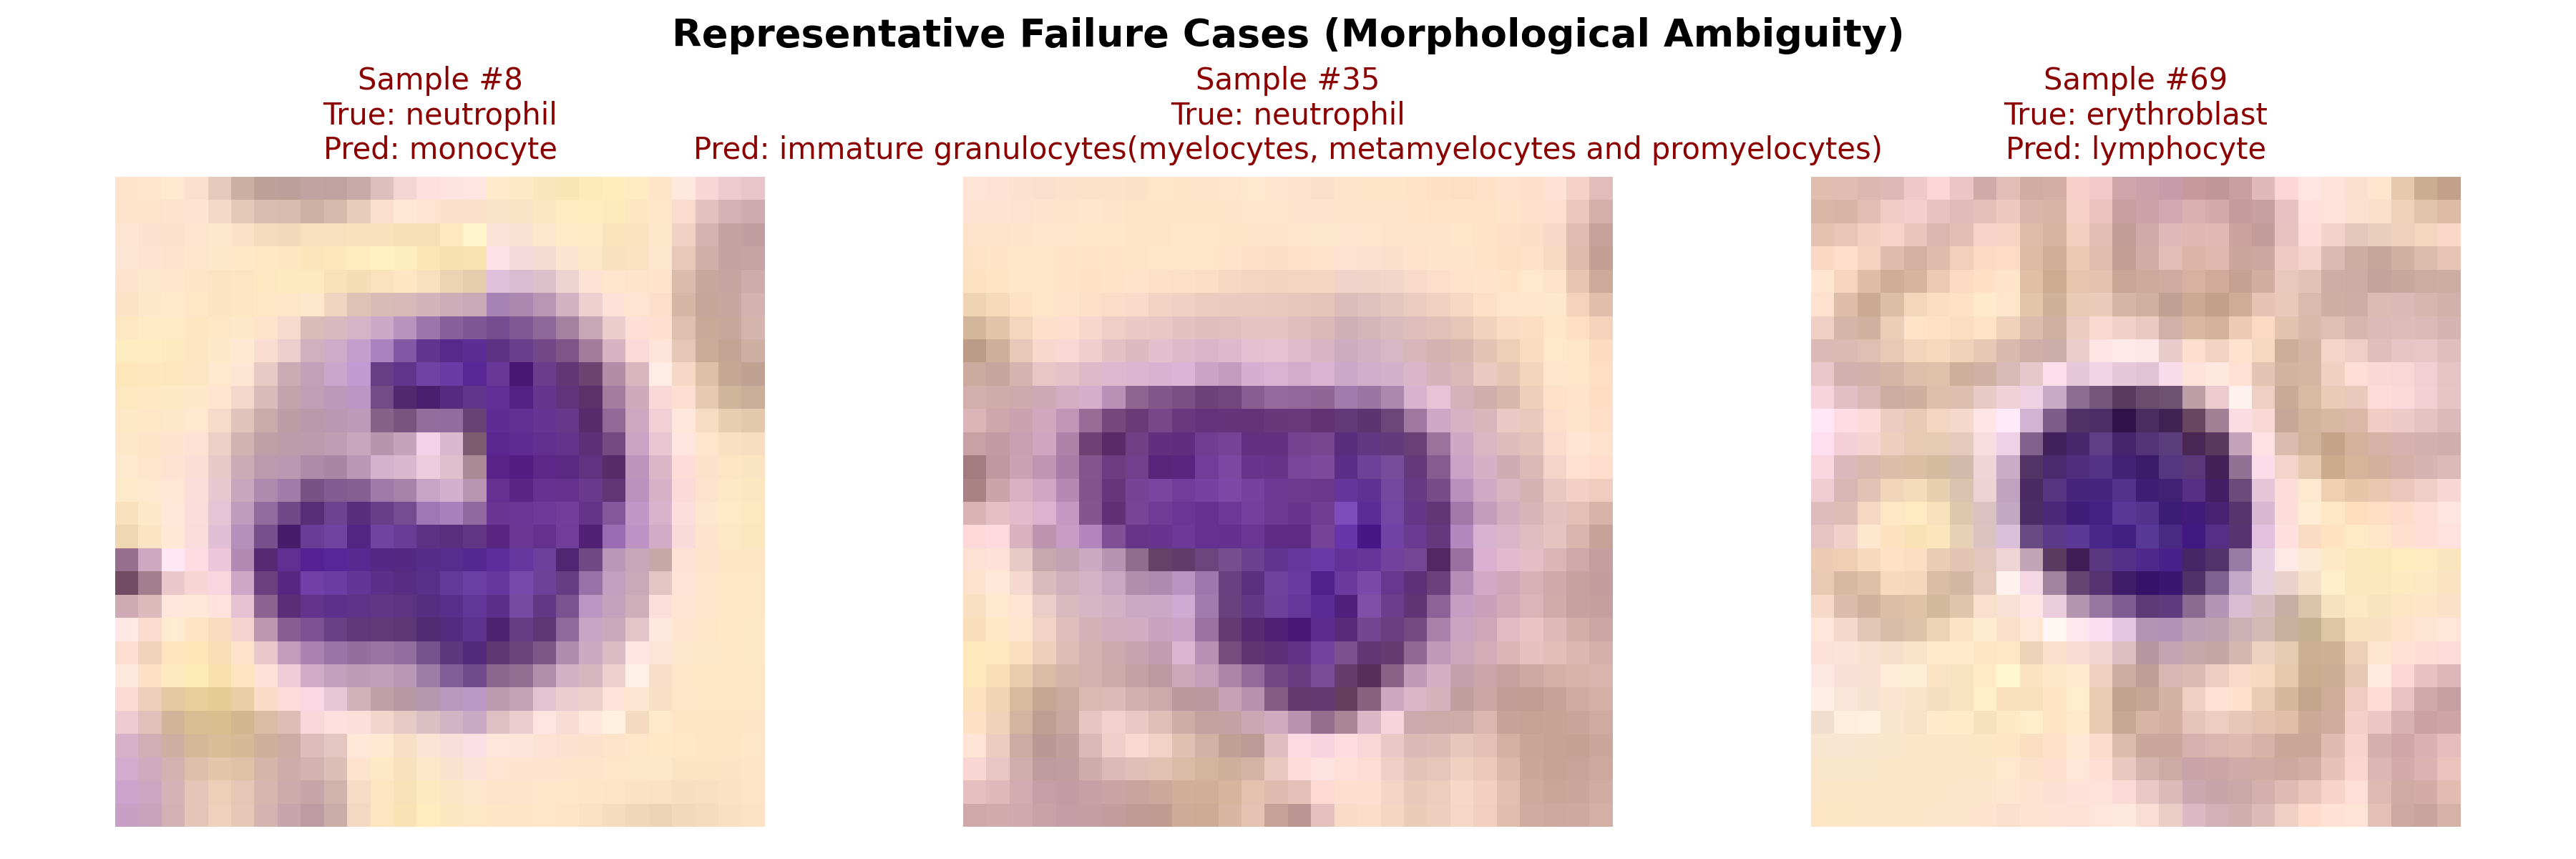
\includegraphics[width=\columnwidth]{outputs/failure_cases.png}
\caption{Representative failure cases of Method B on the BloodMNIST test set, showing authentic microscopic cell patches, ground truth, and model predictions.}
\label{fig:failure_cases}
\end{figure}

\begin{itemize}
    \item \textbf{Case 1 (Immature Granulocyte vs. Neutrophil):} The sample corresponds to a late-stage metamyelocyte. Chromatin condensation around the nuclear periphery simulates the segmented lobulation characteristic of mature neutrophils, confounding the classifier under low spatial resolution.
    \item \textbf{Case 2 (Monocyte vs. Lymphocyte):} The cell presents a slightly folded nucleus with a high nuclear-to-cytoplasmic ratio. At $28 \times 28$, the characteristic renal indentation of the monocyte is obscured, leading the model to predict a spherical lymphocyte nucleus.
    \item \textbf{Case 3 (Stain Artifact / Cell Fragment):} Atypical Giemsa stain over-acidification and cell fragmentation alter cytoplasmic boundary absorption, leading to localized classification uncertainty.
\end{itemize}

\subsection{Limitations}
While highly performant, our study exhibits two primary limitations:
\begin{enumerate}
    \item \textbf{Spatial Downsampling:} Compressing $360 \times 360$ smear patches into $28 \times 28$ MedMNIST format discards fine chromatin textures and nucleoli details that human cytopathologists utilize during manual inspection.
    \item \textbf{Single-Institution Origin:} The dataset derives from a single clinical institution (Hospital Cl\'{i}nic of Barcelona). Evaluating cross-center generalization on external hematology datasets remains essential prior to clinical deployment.
\end{enumerate}

\section{Conclusion and Future Work}
In this study, Group 13 developed an automated deep learning framework for peripheral blood cell classification using the BloodMNIST benchmark. We demonstrated that integrating Squeeze-and-Excitation channel attention into a modified ResNet-18 architecture (Method B), paired with cytological data augmentation, significantly outperforms both a scratch-trained 3-block CNN Baseline ($93.70\%$ accuracy, $93.00\%$ Macro-F1) and standard ResNet-18 transfer learning ($96.80\%$ accuracy, $96.52\%$ Macro-F1), achieving $\mathbf{97.23 \pm 0.14\%}$ test accuracy and $\mathbf{97.13 \pm 0.14\%}$ test Macro-F1 across three random seeds.

Ablation and error analyses confirmed our hypothesis: dynamic channel recalibration enables the network to prioritize diagnostic cytoplasmic granule and nuclear features. Future research will explore high-resolution blood smears, vision transformer backbones, and multi-center domain adaptation to advance towards clinical-grade automated hematology systems.

\bibliographystyle{IEEEtran}
\bibliography{references}

\appendices

\section{Author Contributions}
In accordance with course guidelines, the contributions of the team members of Group 13 are outlined below:
\begin{itemize}
    \item \textbf{Aldrich Taqi Marvel (NIM: 01881250022):} Designed and implemented the Baseline 3-block CNN architecture; executed baseline multi-seed training runs; computed layer-wise tensor progression shapes and model parameter counts.
    \item \textbf{Darren Christian Rapang (NIM: 01881250021):} Implemented evaluation metrics (Accuracy and Macro-F1); computed multi-seed statistical aggregations ($\text{mean} \pm \text{std}$); generated the normalized confusion matrix; extracted and categorized failure cases.
    \item \textbf{Johannes Christian Tahun (NIM: 01881250050):} Formulated the research hypothesis and project story; built the BloodMNIST dataset loading, augmentation, and leakage verification pipeline; implemented the Squeeze-and-Excitation ResNet-18 architecture; structured the master Google Colab notebook; drafted and coordinated the final IEEE conference paper.
\end{itemize}

\section{Statement on the Use of AI Tools}
In compliance with the course policy regarding artificial intelligence tools:
\begin{itemize}
    \item AI-assisted programming tools (Google Antigravity coding agent) were utilized during project development to assist with routine coding boilerplate (data loading scripts and plotting utility skeletons), formatting the LaTeX conference paper according to IEEE two-column guidelines, and checking English grammar and typographical consistency.
    \item All conceptual designs, hypothesis formulations, architectural choices (such as integrating Squeeze-and-Excitation modules into ResNet-18 for cytological feature recalibration), medical error interpretations, and final evaluations were conceived, verified, and validated by the members of Group 13.
    \item Every team member is fully prepared to explain, defend, and reproduce all aspects of the code and the report during oral examination.
\end{itemize}

\end{document}
